%!TEX root = ../thesis.tex
\chapter{Background}
\label{chap:background}


Studying ways to bridge the gap between the fields of \gls{MAS} and \gls{MABS} has been the subject of several works and resulted in the development of different tools, each with its own purpose. Some works were in search of increased performance for MABS; others tried to cater specific needs such as providing an appropriate learning environment. This chapter describes some works that are relevant to this thesis and makes a comparison between some of them. Also included later in this chapter is an overview of code transformation tools that were studied as part of the development of the proposed solution.

\section{Related Work}
% Study of similar frameworks for agent based simulation
Several frameworks exist that offer support to the development of MAS or MABS. Some are domain specific, meaning that their purposed was well defined in their conception. Examples are MASeRaTi\cite{ahlbrecht2014scalable}, MATSim\cite{balmer2008agent} and SUMO\cite{SUMO2012} which are MABS frameworks for traffic and transports simulation. Others like Repast\cite{collier2003repast}, NetLogo\cite{tisue2004netlogo}, GALATEA\cite{davila2000galatea} and Plasma\cite{warden2010towards} are considered general-purpose.This list comprises only tools that are free and open source and is not meant to be exhaustive.

Some works propose approaches that are very similar to the solution proposed in this thesis to solve some of its goals, namely the bridging of the domains of MAS and Simulation. MISIA, JRep and Plasma were built on top of JADE to create a simulation environment based on it. These three works were studied with more detailed due to these similarities.

MISIA's approach, as suggested by Figure \ref{fig:misia}, is to use a middle layer that acts as the bridge between two other layers that interact with JADE and Repast. By extending the agents in Repast and JADE, communicating through a coordinator and synchronizing their state, these agents work as a single one.

\begin{figure}[h]
	\centering
	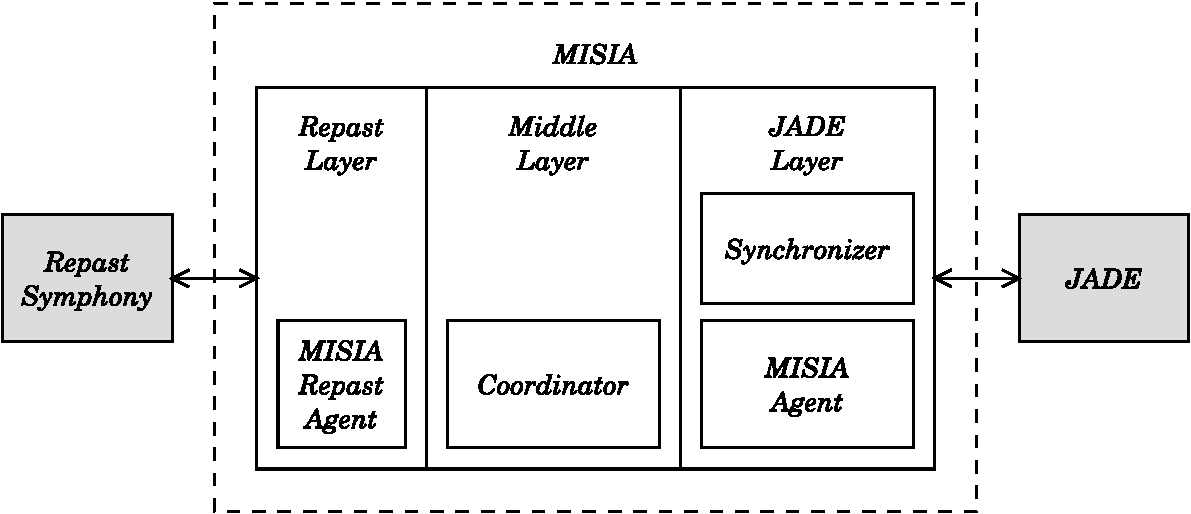
\includegraphics[width=0.75\linewidth]{figures/MISIA.pdf}
	\caption{High-level representation of MISIA's architecture (adapted from \cite{garcia2011misia})}
	\label{fig:misia}
\end{figure}

One of the challenges identified by the authors when re-implementing the FIPA interaction protocols was synchronizing them with the Repast tick-based simulation model. Given JADE's event-driven architecture, MISIA proposes the use of a coordinator agent that informs the JADE-Agent when a tick has passed. It also proposes its own implementation of the interaction protocols supported by JADE, making them tick-friendly.

JReps's approach is not as complex as MISIA's.
By having the Repast Simphony agent encapsulate a JADE agent representation, synchronization is immediate and is assured without requiring an external coordinator.
The two agent representations take care of synchronizing any state changes.
Figure \ref{fig:jrep} represents the basic structure of JRep.

\begin{figure}[h]
	\centering
	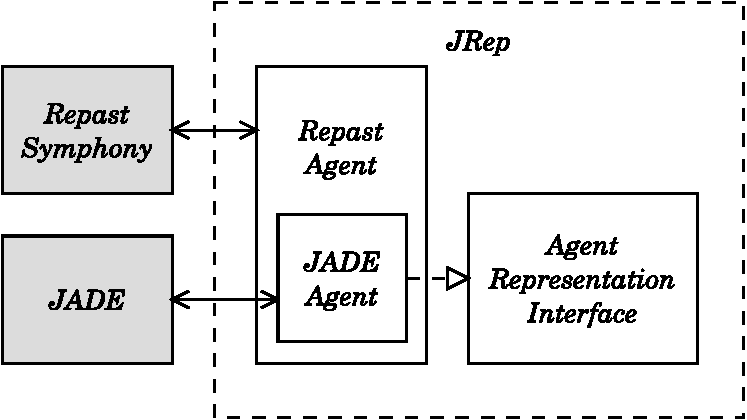
\includegraphics[width=0.5\linewidth]{figures/jrep.pdf}
	\caption{High-level representation of JRep's architecture}
	\label{fig:jrep}
\end{figure}

Each agent takes care of interfacing their respective frameworks. The interaction between agents in JRep is performed using FIPA ACL and the protocol implementations are those provided by the JADE platform. Similarly to MISIA, an Agent Representation Interface is used to introduce the concept of schedule in the JADE agent

Unlike the two previous frameworks, the PlaSMA system is based solely on the JADE platform. The distributed simulation is synchronized by entities called ``Controllers'' who communicate with the ``Top Controller'', keeping the pace of the simulation and handling agent lifecycle management as well. Figure \ref{fig:plasma} illustrates this architecture. PlaSMA, unlike MISIA and JRep, is still an active project - both the other were discontinue and no current deployment of them are available.

\begin{figure}[h]
	\centering
	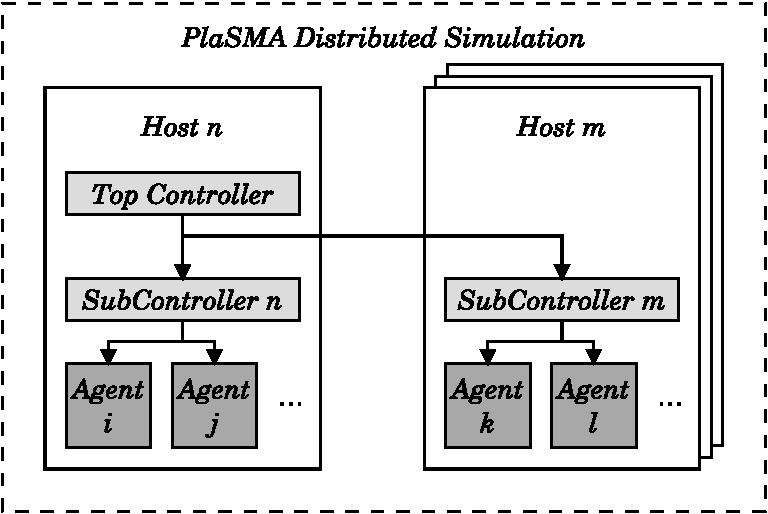
\includegraphics[width=0.5\linewidth]{figures/PlaSMA.pdf}
	\caption{High-level representation of PlaSMA's architecture}
	\label{fig:plasma}
\end{figure}

JADE is a very rich platform but, for many simulation scenarios, the overhead introduced by it has a significant impact on simulation performance \cite{mengistu2008scalability}. \apiname{}, as we describe with more detail in Section \ref{chap:solution}, uses an architecture that is conceptually very close to JADE's but tailored for Repast with no extra dependencies. Moreover, the API could be used with other simulation frameworks with little adaptation.

As suggested by Figure \ref{fig:related-repacl}, \apiname{}'s general structure is simpler than that of JRep and MISIA. Our API does not intend to maintain an active connection to a JADE platform, eliminating the need for synchronization. Instead, our goal is to replicate in our API the main features of JADE, allowing for a straightforward and dependency free feature mapping between our API and JADE.

\begin{figure}
	\centering
	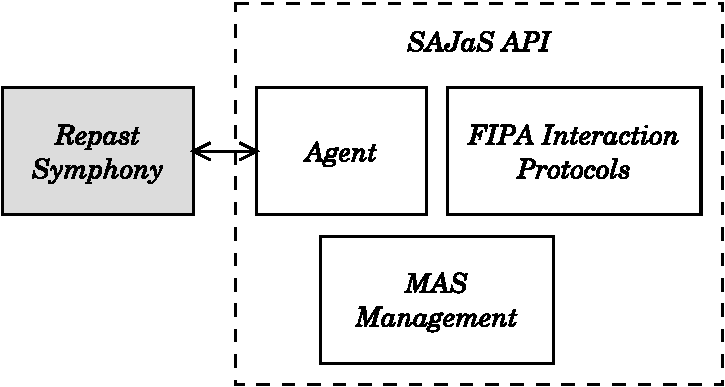
\includegraphics[width=0.5\linewidth]{figures/repacl.pdf}
	\caption{Basic structure of \apiname{}}
	\label{fig:related-repacl}
\end{figure}

Even though both MISIA and JRep attempt to integrate the features from both JADE and Repast, as far as Repast simulations are concerned JADE's multi-threaded infrastructure affects their performance very significantly. The main advantage of our approach is, therefore, the possibility of using Repast with JADE features, namely FIPA specifications including interaction protocols, without the need to interface with JADE. 

\section{Other similar work}
Other works related to integration of features from Repast and JADE are available. While the goal of this thesis is not to use both frameworks simultaneously, these works give a valuable insight into the shortcomings of both frameworks as well as providing some interesting comparisons between their features. 

MISIA and JREP both attempted to complement Repast's lack of communication protocols by creating an interface with JADE's implementation of FIPA interaction protocols. Open source projects exist that contemplate the use of FIPA ACL as a library, but none was found to be actively maintained or properly documented. Therefore, this thesis contemplates the creation of a Java library that brings JADE-like features to simulation tools, including FIPA standards. Chapter \ref{chap:solution} provides a more detailed description of the proposed solution. The next section makes a comparison between JADE and Repast.

\section{JADE and Repast}

To achieve the goals of this thesis, two frameworks were chosen: JADE and Repast. Both are very popular and in widespread use and have been the foundation of the creation of other tools. They are also free and open source and extensively documented.

JADE is a framework for development of FIPA-compliant fully featured MAS. It aims at simplifying the creation of distributed agent applications by seamlessly hiding all complexity regarding its distributed architecture, including the tasks of agent discovery and the handling of messages.

Repast is a toolkit that provides an environment for the creation of MABS using POJO\footnote{Plain Old Java Objects}. It makes it fairly simple to collect agent data and generate displays for it, including charts, grids and others.

\begin{table}[h]
	\caption{Summary of JADE and Repast features.}
	\label{tab:jadevsrep}
	\begin{center}
		\begin{tabular}{l|cc}
		\hline

		\hline
		\textbf{} & \textbf{JADE} & \textbf{Repast} \\ %& \textbf{Cougaar} \\
		\hline
			Communication & FIPA ACL &  Method calls  \\ %& Serialized Object \\
						  &			 &  Shared resources \\
		\hline
			Distribution & Yes & No \\ %& Yes \\
		\hline
			Simulation Tools & No & Yes \\ %& Yes \\
		\hline
			Scalability & Limited & High \\ %& High \\
		\hline
			Ontologies & Yes & No \\ %& Yes\\
		\hline
			Open Source & Yes & Yes \\ %& Yes\\
		\hline
			Agent Execution & Behavior-based & Schedule-based  \\ %&  \\
							& Multi-threaded & Single-threaded \\ %&  \\
							& Event-driven   & Tick-driven 	   \\ %&  \\
							& Assync		 & Sync 		   \\ %&  \\
		\hline
		\end{tabular}
	\end{center}
\end{table}

In JADE, as table \ref{tab:jadevsrep} illustrates, agents execute in separate threads and while this architecture facilitates the platform's distribution, JADE's agent are heavy in terms of resources. Experiments with JADE show that the platform's scalability is limited in number of agents and that the global system performance drops quickly for large number of agents \cite{mengistu2008scalability} \cite{garcia2011misia}. This further strengthens the idea that using JADE or a JADE-Repast hybrid, as describe in the related work, is not the best course of action is performance is an important issue.


\section{Code generation}

The proposed solution includes more than simple integration of JADE-like features in simulation tools like Repast. Methodologies of code transformation were studied to allow automatic generation of a simulation from a MAS or vice versa.

There are multiple ways to tackle the problem of code transformations, as described in this thesis. The brute force approach would be to parse the source code, create an abstract syntax tree (AST), which represents all code constructions in a program, perform certain transformations in the tree, and then generate back the code from the new AST. Fortunately, there are free and open source projects that developers can use to do exactly this with significantly reduced effort. From the available tools, I selected the ones that are the most relevant to this thesis, i.e. tools for Java code transformation that are open source, well documented and still supported.


\subsection{Spoon - Program Analysis and Transformation in Java}
	Spoon is a tool created to take advantage of the new features introduced on the release of Java 5, namely annotations and generics. It is a Java transformation tool that uses annotation processing, compile-time reflection and templates in a pure-Java environment to enable programmers to create their own platforms for code transformations. These transformations occur on compile time and annotations are used as parameters for compilation. The programmer uses plain Java code to define the transformations that should occur, for instance, adding code snippets to the beginning of a method in a class. Finally, Spoon can be seamlessly integrated in an IDE such as Eclipse \cite{pawlak2006spoon}.


\subsection{ATL - ATL Transformation Language }
	ATL - \emph{ATLAS Transformation Language}, is both the name of a language and its enclosing plug-in and allows the creation of model transformations. Unlike JDT and Spoon analyzed before, ATL does not focus on applying transformations to the source code.

	As explained in Jouault \emph{et al}, ``a source model Ma is transformed into a target model Mb according to a transformation definition mma2mmb.atl written in the ATL language'', which is also a model itself. The three must conform to their respective metamodels MMa, MMb and ATL which then conform to the metametamodel MOF.
% end % Code generation tools

\subsection{Eclipse Java Development Tools (JDT)}

	The Java Development Tools\footnote{https://www.eclipse.org/jdt/} are are a group of tools that provide Eclipse the necessary means to become a full-featured Java IDE.
	These tools make up what we perceive as the ``Eclipse IDE'' and programmers can use these libraries in their Java projects and perform tasks that require a certain introspection of the code itself. 

	JDT was chosen for the development of the code generation tool. Some of its most interesting features are the automatic cloning of projects, the handling of classes, imports, methods and fields as objects and the possibility of doing complex manipulation tasks without parsing the code. It does, however, allow the use of a high level AST for a more direct manipulation of the source code.

	JDT can be broken down into five main components: 

	\begin{description}
		\item[APT] - Annotation Processing Tool\hfill \\
  			This component can be used to parse annotations in the code. Annotations are a Java construction introduced in Java 5 and can be used to add meta information about classes, objects and methods. These annotations can then be parsed by frameworks that use the POJO that enclose them.
		\item[Core] - Java IDE headless infrastructure \hfill \\
  			The core for the Java IDE, it allows to transverse the Java element tree and find package fragments, compilation units, binary classes, types, methods and fields. This is the most extensively used component by the code transformation tool.
		\item[Debug] - Debug support for Java\hfill \\
  			This tool makes the debug facilities of Eclipse possible. It provides functionalities such as execution control and contextual expression evaluation.
		\item[Text and UI] - Java editing support and Java IDE user interface \hfill \\
  			These components make development in Eclipse possible by providing a GUI for code editing, enriched with syntactic errors highlighting, among other interesting aids.
	\end{description}

%!TEX root = ../thesis.tex
\section{FIPA Specifications in JADE} % (fold)
\label{sec:fipa}

% Intro to FIPA in JADE/API
\apiname{} closely follows JADE's architecture regarding the use of protocols and services specified by FIPA. 
%The architecture of the API described in this paper includes multiple concepts proposed by FIPA: the \gls{DF}, the \gls{MTS}, the \gls{AMS}, the \gls{ACL} Message and the Interaction Protocols. The following is a brief description of these concepts and of how JADE uses and implements them.

%\begin{figure}
%	\centering
%	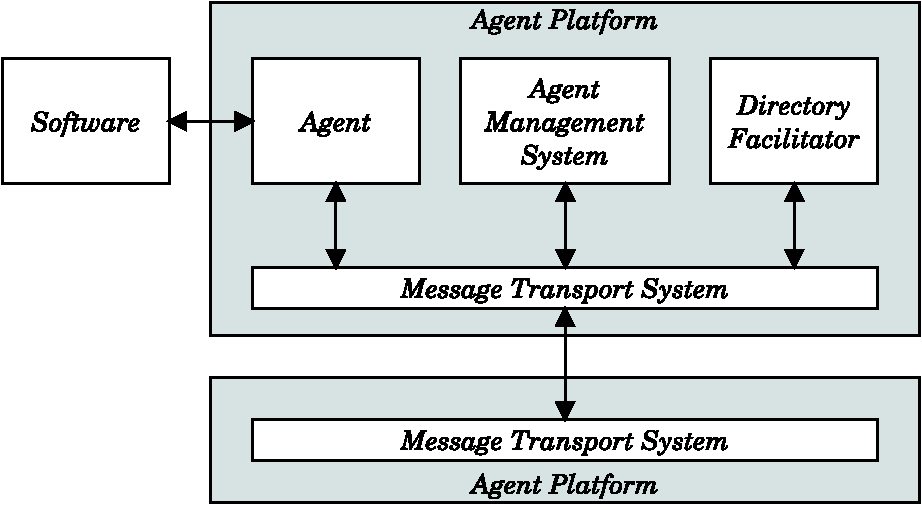
\includegraphics[width=2.5in]{figures/pdf/AMSdiagram.pdf}
%	\caption{
%		Agent Management Reference Model, as specified by FIPA and implemented by JADE. \apiname{} only supports a single Agent Platform.
%	}
%	\label{fig:AMSdiagram}
%\end{figure}

% DF 
The Directory Service (DF) is a component that provides a yellow page service and is part of the FIPA Agent Management Specification. It allows one agent to perform searches about agents rendering specific services. Only agents that are registered in the DF will be indexed and agents can register and deregister themselves at any time.

% DF Agent Description
When searching the DF, agents can use templates that filter the search results. A DF Agent Description represents this template and contains the fields listed in Table \ref{tab:dfAgentDescription}.sim


% MTS
The MTS is a service for transportation of ACL messages between agents. It is responsible for resolving agent addresses, in order to be able to deliver those messages. The MTS may request information from the AMS to perform this address resolution.

% AMS
The AMS is a mandatory component in FIPA-compliant agent platforms. Its purpose is to manage the agent platform, namely the creating and deletion of agents.

% ACL Message
The ACL Message is the envelope that contains the details for communication. The Agent Comunication Language (ACL) stipulates what fields a message should contain. Table \ref{tab:fipaACLMessage} was adapted from the FIPA ACL Message structure specification and contains the list of fields in a message. Not all of them are mandatory. FIPA specifies the \texttt{performative} as the only mandatory field, although the \texttt{sender}, \texttt{receiver} and \texttt{content} are expected to be present.

\begin{table}
	\normalsize
	\caption{FIPA ACL Message Parameters}
	\label{tab:fipaACLMessage}
	\begin{center}
		\fboxsep1pt
		\begin{tabular}{c|c}
		\hline
		\textbf{Parameter} & \textbf{Category of Parameters} \\
		\hline
		\colorbox{Apricot}{\texttt{performative}} & Type of communicative acts \\
		\hline
		\colorbox{Apricot}{\texttt{sender}} & \multirow{3}{*}{Participant in communication} \\
		\cline{1-1}
		\colorbox{Apricot}{\texttt{receiver}} \\
		\cline{1-1}
		\texttt{reply-to}  \\
		\hline
		\colorbox{Apricot}{\texttt{content}} & Content of message \\
		\hline
		\texttt{language} & \multirow{3}{*}{Description of Content} \\
		\cline{1-1}
		\texttt{encoding} \\
		\cline{1-1}
		\colorbox{Apricot}{\texttt{ontology}} \\
		\hline
		\colorbox{Apricot}{\texttt{protocol}} & \multirow{5}{*}{Control of conversation} \\
		\cline{1-1}
		\colorbox{Apricot}{\texttt{conversation-id}} \\
		\cline{1-1}
		\texttt{reply-with} \\
		\cline{1-1}
		\texttt{in-reply-to} \\
		\cline{1-1}
		\colorbox{Apricot}{\texttt{reply-by}} \\
		\hline
		\end{tabular}
	\end{center}
\end{table} 

% Protocols In FIPA
FIPA Interaction Protocols typify communication interactions among agents by specifying two roles: initiator (the agent starting the interaction) and responder (a participant in the interaction). Each protocol defines precisely which messages are sent by each role ad in which sequence.

% Behaviors in JADE
In JADE, every agent activity is programmed through the notion o behaviours. For interaction protocols, typically behaviour-pairs are used for each side of the interaction, and JADE's API supports the most important protocols with built-in initiator and responder behaviours.
% Implementing these protocols.
In order to create an application using these protocols, programmers only need to extend these behaviours and implement the message handlers.
All the complexity regarding the interaction and networking infrastructure is hidden and taken care of by JADE, allowing the programmer to focus on the implementation of agent behaviour.

\subsection{FIPA Interaction Protocols}

To provide a more solid background to the protocols mentioned in this thesis, it's relevant to perform a deeper analysys of them. The two protocols currently supported in the API, as will be explained further ahead in Chapter \ref{chap:solution}, are the FIPA Request, FIPA Query and the FIPA Contract Net. JADE supports a few other protocols, namely FIPA Propose, Iterated FIPA Request and Query and FIPA Subscribe.

\begin{table}
	\normalsize
	\caption{Interaction protocols supported in JADE}
	\label{tab:fipa_protos}
	\begin{center}
		\fboxsep1pt
		\begin{tabular}{c|c|c}
		\hline
		\textbf{Protocol(s)} & \textbf{Initiator class} & \textbf{Initiator class} \\
		\hline
		FIPA request 	& \multirow{2}{*}{AchieveREInitiator} & \multirow{2}{*}{AchieveREResponder}\\
		FIPA Query 		& \\
		\hline
		\multirow{2}{*}{FIPA Contract Net} & \multirow{2}{*}{ContractNetInitiator} & ContractNetResponder \\
		 &  & SSContractNetResponder \\
		\hline
		\end{tabular}
	\end{center}
\end{table}


In JADE, the AchieveRE protocol encompases the multiple ``request-like'' behaviours such as FIPA-Request. It is a simple protocol with three moments of interaction, as Figure \ref{fig:FIPA_request_proto} shows: a request, a response of acceptance or refusal and a facultative result notification. JADE allows the use of other interaction protocols with the AchieveRE: FIPA-query, FIPA-Request-When, FIPA-recruiting and FIPA-brokering. Interaction using this protocol can be 1:1 or 1:N.

The Contract Net protocol starts with a Call for Proposals (CFP) sent to one or more agents, which can reply with a proposal or with a refusal to propose. The initiator can then accept or reject the proposals. As in FIPA-Request, the final result notification is facultative. The ContractNetResponder class from JADE resets itself after terminating the protocol and stays waiting for new CFPs. JADE provides an alternative responder class called SSContractNetResponder that terminates after a single session (SS stands for single session).

\begin{figure}[ht]
	\centering
    \begin{subfigure}[b]{0.44\textwidth}
		\centering
		\includegraphics[height=4in]{figures/FIPA_request_proto.pdf}
		\caption[FIPA-Request protocol]{FIPA-Request protocol}
		\label{fig:FIPA_request_proto}
    \end{subfigure}%
    \begin{subfigure}[b]{0.54\textwidth}
		\centering
		\includegraphics[height=4in]{figures/FIPA_contnet_proto.pdf}
		\caption[FIPA-Contract-Net protocol]{FIPA-Contract-Net protocol}
		\label{fig:FIPA_contnet_proto}
    \end{subfigure}
    \caption[]{Sequence diagrams for the protocols Contract Net and Request. \\Figures are from the FIPA specifications website \footnote{http://fipa.org/})}
    \label{fig:FIPA_Protocols}
\end{figure}


\section{Summary}
Although the specific problem of converting code between JADE and Repast has not been approached before in the available literature, it is clear that some related work is useful in the definition of the solution proposed in this thesis. JREP and MISIA show is that interoperability between the two frameworks is possible and they helped understand the limitations of each framework. The usefulness of these works is limited, though, since the source code is not readily available and neither project is still being developed and supported. Also, one of the goals proposed in the Introduction refers to the ability to generate code with introducing extensive changes to the original code. What JREP and MISIA propose is a platform to build new systems from scratch using JADE and Repast simultaneously. The next chapters give a thorough explanation of the developed solution.